% Options for packages loaded elsewhere
\PassOptionsToPackage{unicode}{hyperref}
\PassOptionsToPackage{hyphens}{url}
\PassOptionsToPackage{dvipsnames,svgnames,x11names}{xcolor}
%
\documentclass[
  letterpaper,
  DIV=11,
  numbers=noendperiod]{scrartcl}

\usepackage{amsmath,amssymb}
\usepackage{iftex}
\ifPDFTeX
  \usepackage[T1]{fontenc}
  \usepackage[utf8]{inputenc}
  \usepackage{textcomp} % provide euro and other symbols
\else % if luatex or xetex
  \usepackage{unicode-math}
  \defaultfontfeatures{Scale=MatchLowercase}
  \defaultfontfeatures[\rmfamily]{Ligatures=TeX,Scale=1}
\fi
\usepackage{lmodern}
\ifPDFTeX\else  
    % xetex/luatex font selection
\fi
% Use upquote if available, for straight quotes in verbatim environments
\IfFileExists{upquote.sty}{\usepackage{upquote}}{}
\IfFileExists{microtype.sty}{% use microtype if available
  \usepackage[]{microtype}
  \UseMicrotypeSet[protrusion]{basicmath} % disable protrusion for tt fonts
}{}
\makeatletter
\@ifundefined{KOMAClassName}{% if non-KOMA class
  \IfFileExists{parskip.sty}{%
    \usepackage{parskip}
  }{% else
    \setlength{\parindent}{0pt}
    \setlength{\parskip}{6pt plus 2pt minus 1pt}}
}{% if KOMA class
  \KOMAoptions{parskip=half}}
\makeatother
\usepackage{xcolor}
\usepackage{soul}
\setlength{\emergencystretch}{3em} % prevent overfull lines
\setcounter{secnumdepth}{-\maxdimen} % remove section numbering
% Make \paragraph and \subparagraph free-standing
\ifx\paragraph\undefined\else
  \let\oldparagraph\paragraph
  \renewcommand{\paragraph}[1]{\oldparagraph{#1}\mbox{}}
\fi
\ifx\subparagraph\undefined\else
  \let\oldsubparagraph\subparagraph
  \renewcommand{\subparagraph}[1]{\oldsubparagraph{#1}\mbox{}}
\fi

\usepackage{color}
\usepackage{fancyvrb}
\newcommand{\VerbBar}{|}
\newcommand{\VERB}{\Verb[commandchars=\\\{\}]}
\DefineVerbatimEnvironment{Highlighting}{Verbatim}{commandchars=\\\{\}}
% Add ',fontsize=\small' for more characters per line
\usepackage{framed}
\definecolor{shadecolor}{RGB}{241,243,245}
\newenvironment{Shaded}{\begin{snugshade}}{\end{snugshade}}
\newcommand{\AlertTok}[1]{\textcolor[rgb]{0.68,0.00,0.00}{#1}}
\newcommand{\AnnotationTok}[1]{\textcolor[rgb]{0.37,0.37,0.37}{#1}}
\newcommand{\AttributeTok}[1]{\textcolor[rgb]{0.40,0.45,0.13}{#1}}
\newcommand{\BaseNTok}[1]{\textcolor[rgb]{0.68,0.00,0.00}{#1}}
\newcommand{\BuiltInTok}[1]{\textcolor[rgb]{0.00,0.23,0.31}{#1}}
\newcommand{\CharTok}[1]{\textcolor[rgb]{0.13,0.47,0.30}{#1}}
\newcommand{\CommentTok}[1]{\textcolor[rgb]{0.37,0.37,0.37}{#1}}
\newcommand{\CommentVarTok}[1]{\textcolor[rgb]{0.37,0.37,0.37}{\textit{#1}}}
\newcommand{\ConstantTok}[1]{\textcolor[rgb]{0.56,0.35,0.01}{#1}}
\newcommand{\ControlFlowTok}[1]{\textcolor[rgb]{0.00,0.23,0.31}{#1}}
\newcommand{\DataTypeTok}[1]{\textcolor[rgb]{0.68,0.00,0.00}{#1}}
\newcommand{\DecValTok}[1]{\textcolor[rgb]{0.68,0.00,0.00}{#1}}
\newcommand{\DocumentationTok}[1]{\textcolor[rgb]{0.37,0.37,0.37}{\textit{#1}}}
\newcommand{\ErrorTok}[1]{\textcolor[rgb]{0.68,0.00,0.00}{#1}}
\newcommand{\ExtensionTok}[1]{\textcolor[rgb]{0.00,0.23,0.31}{#1}}
\newcommand{\FloatTok}[1]{\textcolor[rgb]{0.68,0.00,0.00}{#1}}
\newcommand{\FunctionTok}[1]{\textcolor[rgb]{0.28,0.35,0.67}{#1}}
\newcommand{\ImportTok}[1]{\textcolor[rgb]{0.00,0.46,0.62}{#1}}
\newcommand{\InformationTok}[1]{\textcolor[rgb]{0.37,0.37,0.37}{#1}}
\newcommand{\KeywordTok}[1]{\textcolor[rgb]{0.00,0.23,0.31}{#1}}
\newcommand{\NormalTok}[1]{\textcolor[rgb]{0.00,0.23,0.31}{#1}}
\newcommand{\OperatorTok}[1]{\textcolor[rgb]{0.37,0.37,0.37}{#1}}
\newcommand{\OtherTok}[1]{\textcolor[rgb]{0.00,0.23,0.31}{#1}}
\newcommand{\PreprocessorTok}[1]{\textcolor[rgb]{0.68,0.00,0.00}{#1}}
\newcommand{\RegionMarkerTok}[1]{\textcolor[rgb]{0.00,0.23,0.31}{#1}}
\newcommand{\SpecialCharTok}[1]{\textcolor[rgb]{0.37,0.37,0.37}{#1}}
\newcommand{\SpecialStringTok}[1]{\textcolor[rgb]{0.13,0.47,0.30}{#1}}
\newcommand{\StringTok}[1]{\textcolor[rgb]{0.13,0.47,0.30}{#1}}
\newcommand{\VariableTok}[1]{\textcolor[rgb]{0.07,0.07,0.07}{#1}}
\newcommand{\VerbatimStringTok}[1]{\textcolor[rgb]{0.13,0.47,0.30}{#1}}
\newcommand{\WarningTok}[1]{\textcolor[rgb]{0.37,0.37,0.37}{\textit{#1}}}

\providecommand{\tightlist}{%
  \setlength{\itemsep}{0pt}\setlength{\parskip}{0pt}}\usepackage{longtable,booktabs,array}
\usepackage{calc} % for calculating minipage widths
% Correct order of tables after \paragraph or \subparagraph
\usepackage{etoolbox}
\makeatletter
\patchcmd\longtable{\par}{\if@noskipsec\mbox{}\fi\par}{}{}
\makeatother
% Allow footnotes in longtable head/foot
\IfFileExists{footnotehyper.sty}{\usepackage{footnotehyper}}{\usepackage{footnote}}
\makesavenoteenv{longtable}
\usepackage{graphicx}
\makeatletter
\def\maxwidth{\ifdim\Gin@nat@width>\linewidth\linewidth\else\Gin@nat@width\fi}
\def\maxheight{\ifdim\Gin@nat@height>\textheight\textheight\else\Gin@nat@height\fi}
\makeatother
% Scale images if necessary, so that they will not overflow the page
% margins by default, and it is still possible to overwrite the defaults
% using explicit options in \includegraphics[width, height, ...]{}
\setkeys{Gin}{width=\maxwidth,height=\maxheight,keepaspectratio}
% Set default figure placement to htbp
\makeatletter
\def\fps@figure{htbp}
\makeatother
\newlength{\cslhangindent}
\setlength{\cslhangindent}{1.5em}
\newlength{\csllabelwidth}
\setlength{\csllabelwidth}{3em}
\newlength{\cslentryspacingunit} % times entry-spacing
\setlength{\cslentryspacingunit}{\parskip}
\newenvironment{CSLReferences}[2] % #1 hanging-ident, #2 entry spacing
 {% don't indent paragraphs
  \setlength{\parindent}{0pt}
  % turn on hanging indent if param 1 is 1
  \ifodd #1
  \let\oldpar\par
  \def\par{\hangindent=\cslhangindent\oldpar}
  \fi
  % set entry spacing
  \setlength{\parskip}{#2\cslentryspacingunit}
 }%
 {}
\usepackage{calc}
\newcommand{\CSLBlock}[1]{#1\hfill\break}
\newcommand{\CSLLeftMargin}[1]{\parbox[t]{\csllabelwidth}{#1}}
\newcommand{\CSLRightInline}[1]{\parbox[t]{\linewidth - \csllabelwidth}{#1}\break}
\newcommand{\CSLIndent}[1]{\hspace{\cslhangindent}#1}

\usepackage{booktabs}
\usepackage{longtable}
\usepackage{array}
\usepackage{multirow}
\usepackage{wrapfig}
\usepackage{float}
\usepackage{colortbl}
\usepackage{pdflscape}
\usepackage{tabu}
\usepackage{threeparttable}
\usepackage{threeparttablex}
\usepackage[normalem]{ulem}
\usepackage{makecell}
\usepackage{xcolor}
\KOMAoption{captions}{tableheading}
\makeatletter
\@ifpackageloaded{tcolorbox}{}{\usepackage[skins,breakable]{tcolorbox}}
\@ifpackageloaded{fontawesome5}{}{\usepackage{fontawesome5}}
\definecolor{quarto-callout-color}{HTML}{909090}
\definecolor{quarto-callout-note-color}{HTML}{0758E5}
\definecolor{quarto-callout-important-color}{HTML}{CC1914}
\definecolor{quarto-callout-warning-color}{HTML}{EB9113}
\definecolor{quarto-callout-tip-color}{HTML}{00A047}
\definecolor{quarto-callout-caution-color}{HTML}{FC5300}
\definecolor{quarto-callout-color-frame}{HTML}{acacac}
\definecolor{quarto-callout-note-color-frame}{HTML}{4582ec}
\definecolor{quarto-callout-important-color-frame}{HTML}{d9534f}
\definecolor{quarto-callout-warning-color-frame}{HTML}{f0ad4e}
\definecolor{quarto-callout-tip-color-frame}{HTML}{02b875}
\definecolor{quarto-callout-caution-color-frame}{HTML}{fd7e14}
\makeatother
\makeatletter
\makeatother
\makeatletter
\makeatother
\makeatletter
\@ifpackageloaded{caption}{}{\usepackage{caption}}
\AtBeginDocument{%
\ifdefined\contentsname
  \renewcommand*\contentsname{Table of contents}
\else
  \newcommand\contentsname{Table of contents}
\fi
\ifdefined\listfigurename
  \renewcommand*\listfigurename{List of Figures}
\else
  \newcommand\listfigurename{List of Figures}
\fi
\ifdefined\listtablename
  \renewcommand*\listtablename{List of Tables}
\else
  \newcommand\listtablename{List of Tables}
\fi
\ifdefined\figurename
  \renewcommand*\figurename{Figure}
\else
  \newcommand\figurename{Figure}
\fi
\ifdefined\tablename
  \renewcommand*\tablename{Table}
\else
  \newcommand\tablename{Table}
\fi
}
\@ifpackageloaded{float}{}{\usepackage{float}}
\floatstyle{ruled}
\@ifundefined{c@chapter}{\newfloat{codelisting}{h}{lop}}{\newfloat{codelisting}{h}{lop}[chapter]}
\floatname{codelisting}{Listing}
\newcommand*\listoflistings{\listof{codelisting}{List of Listings}}
\makeatother
\makeatletter
\@ifpackageloaded{caption}{}{\usepackage{caption}}
\@ifpackageloaded{subcaption}{}{\usepackage{subcaption}}
\makeatother
\makeatletter
\@ifpackageloaded{tcolorbox}{}{\usepackage[skins,breakable]{tcolorbox}}
\makeatother
\makeatletter
\@ifundefined{shadecolor}{\definecolor{shadecolor}{rgb}{.97, .97, .97}}
\makeatother
\makeatletter
\makeatother
\makeatletter
\makeatother
\makeatletter
\@ifpackageloaded{tikz}{}{\usepackage{tikz}}
\makeatother
        \newcommand*\circled[1]{\tikz[baseline=(char.base)]{
          \node[shape=circle,draw,inner sep=1pt] (char) {{\scriptsize#1}};}}  
                  
\ifLuaTeX
\usepackage[bidi=basic]{babel}
\else
\usepackage[bidi=default]{babel}
\fi
\babelprovide[main,import]{english}
% get rid of language-specific shorthands (see #6817):
\let\LanguageShortHands\languageshorthands
\def\languageshorthands#1{}
\ifLuaTeX
  \usepackage{selnolig}  % disable illegal ligatures
\fi
\IfFileExists{bookmark.sty}{\usepackage{bookmark}}{\usepackage{hyperref}}
\IfFileExists{xurl.sty}{\usepackage{xurl}}{} % add URL line breaks if available
\urlstyle{same} % disable monospaced font for URLs
\hypersetup{
  pdftitle={Linear Regression 1},
  pdfauthor={Daniela Palleschi},
  pdflang={en},
  colorlinks=true,
  linkcolor={blue},
  filecolor={Maroon},
  citecolor={Blue},
  urlcolor={Blue},
  pdfcreator={LaTeX via pandoc}}

\title{Linear Regression 1}
\usepackage{etoolbox}
\makeatletter
\providecommand{\subtitle}[1]{% add subtitle to \maketitle
  \apptocmd{\@title}{\par {\large #1 \par}}{}{}
}
\makeatother
\subtitle{Simple Linear Regression}
\author{Daniela Palleschi}
\date{2023-04-13}

\begin{document}
\maketitle
\ifdefined\Shaded\renewenvironment{Shaded}{\begin{tcolorbox}[interior hidden, sharp corners, boxrule=0pt, breakable, enhanced, frame hidden, borderline west={3pt}{0pt}{shadecolor}]}{\end{tcolorbox}}\fi

\renewcommand*\contentsname{Table of contents}
{
\hypersetup{linkcolor=}
\setcounter{tocdepth}{3}
\tableofcontents
}
\begin{Shaded}
\begin{Highlighting}[]
\DocumentationTok{\#\# play sound if error encountered}
\DocumentationTok{\#\#\# from: https://sejohnston.com/2015/02/24/make{-}r{-}beep{-}when{-}r{-}markdown{-}finishes{-}or{-}when{-}it{-}fails/}
\FunctionTok{options}\NormalTok{(}\AttributeTok{error =} \ControlFlowTok{function}\NormalTok{()\{    }\CommentTok{\# Beep on error}
\NormalTok{  beepr}\SpecialCharTok{::}\FunctionTok{beep}\NormalTok{(}\AttributeTok{sound =} \StringTok{"wilhelm"}\NormalTok{)}
  \FunctionTok{Sys.sleep}\NormalTok{(}\DecValTok{2}\NormalTok{) }\CommentTok{\# }
\NormalTok{  \}}
\NormalTok{ )}
\DocumentationTok{\#\# and when knitting is complete}
\NormalTok{.Last }\OtherTok{\textless{}{-}} \ControlFlowTok{function}\NormalTok{() \{          }\CommentTok{\# Beep on exiting session}
\NormalTok{  beepr}\SpecialCharTok{::}\FunctionTok{beep}\NormalTok{(}\AttributeTok{sound =} \StringTok{"ping"}\NormalTok{)}
  \FunctionTok{Sys.sleep}\NormalTok{(}\DecValTok{6}\NormalTok{) }\CommentTok{\# allow to play for 6 seconds}
\NormalTok{  \}}
\end{Highlighting}
\end{Shaded}

\begin{Shaded}
\begin{Highlighting}[]
\CommentTok{\# Create references.json file based on the citations in this script}
\CommentTok{\# make sure you have \textquotesingle{}bibliography: references.json\textquotesingle{} in the YAML}
\NormalTok{rbbt}\SpecialCharTok{::}\FunctionTok{bbt\_update\_bib}\NormalTok{(}\StringTok{"\_lin\_reg1.qmd"}\NormalTok{)}
\end{Highlighting}
\end{Shaded}

\begin{verbatim}
Wrote 5 references to './references/references.json'
\end{verbatim}

\begin{Shaded}
\begin{Highlighting}[]
\NormalTok{knitr}\SpecialCharTok{::}\NormalTok{opts\_chunk}\SpecialCharTok{$}\FunctionTok{set}\NormalTok{(}\AttributeTok{eval =}\NormalTok{ T, }\CommentTok{\# change this to \textquotesingle{}eval = T\textquotesingle{} to reproduce the analyses; make sure to comment out}
                      \AttributeTok{echo =}\NormalTok{ T, }\CommentTok{\# \textquotesingle{}print code chunk?\textquotesingle{}}
                      \AttributeTok{message =}\NormalTok{ F, }\CommentTok{\# \textquotesingle{}print messages (e.g., warnings)?\textquotesingle{}}
                      \AttributeTok{error =}\NormalTok{ F,}
                      \AttributeTok{warning =}\NormalTok{ F)}
\end{Highlighting}
\end{Shaded}

\hypertarget{set-up-environment}{%
\section{Set-up environment}\label{set-up-environment}}

\begin{Shaded}
\begin{Highlighting}[]
\CommentTok{\# suppress scientific notation}
\FunctionTok{options}\NormalTok{(}\AttributeTok{scipen=}\DecValTok{999}\NormalTok{)}

\CommentTok{\# load libraries}
\FunctionTok{library}\NormalTok{(tidyverse)}
\FunctionTok{library}\NormalTok{(ggplot2)}
\FunctionTok{library}\NormalTok{(broom)}
\end{Highlighting}
\end{Shaded}

\begin{Shaded}
\begin{Highlighting}[]
\CommentTok{\# load in dataset}
\NormalTok{df\_crit\_verb }\OtherTok{\textless{}{-}}\NormalTok{ readr}\SpecialCharTok{::}\FunctionTok{read\_csv}\NormalTok{(here}\SpecialCharTok{::}\FunctionTok{here}\NormalTok{(}\StringTok{"data/tidy\_data\_lifetime\_pilot.csv"}\NormalTok{), }
                               \CommentTok{\# for special characters}
                               \AttributeTok{locale =}\NormalTok{ readr}\SpecialCharTok{::}\FunctionTok{locale}\NormalTok{(}\AttributeTok{encoding =} \StringTok{"latin1"}\NormalTok{) }
\NormalTok{                               ) }\SpecialCharTok{|\textgreater{}} 
  \FunctionTok{mutate\_if}\NormalTok{(is.character,as.factor) }\SpecialCharTok{|\textgreater{}} \CommentTok{\# all character variables as factor}
  \FunctionTok{filter}\NormalTok{(type }\SpecialCharTok{==} \StringTok{"critical"}\NormalTok{, }\CommentTok{\# only critical trials}
\NormalTok{         px }\SpecialCharTok{!=} \StringTok{"px7"}\NormalTok{, }\CommentTok{\# px7 had a lot of missing values}
\NormalTok{         region }\SpecialCharTok{==} \StringTok{"verb"}\NormalTok{) }\CommentTok{\# critical region only}
\end{Highlighting}
\end{Shaded}

\hypertarget{resources}{%
\section{Resources}\label{resources}}

\begin{itemize}
\tightlist
\item
  these slides are based on a mix of the following resources
\end{itemize}

DeBruine \& Barr (2021); Winter (2013); Winter (2014); Winter (2019)

\begin{itemize}
\tightlist
\item
  and on slides that were originally based on Field et al. (2013), but
  if you're looking for a textbook I'd recommend Winter (2019)
\end{itemize}

\hypertarget{linear-regression}{%
\section{(Linear) Regression}\label{linear-regression}}

\begin{itemize}
\tightlist
\item
  our data exploration has given us an idea about what our data look
  like
\item
  we fit a model to our data, and use it to \emph{predict} values of our
  DV based on one (or more) IV(s)

  \begin{itemize}
  \tightlist
  \item
    i.e., \emph{predicting} an outcome variable (DIV) from one or more
    predictors (IVs)
  \end{itemize}
\item
  because we're making predictions, we need to take into account the
  variability (i.e., \emph{error}) in our data
\end{itemize}

\begin{tcolorbox}[enhanced jigsaw, leftrule=.75mm, bottomrule=.15mm, breakable, left=2mm, colback=white, bottomtitle=1mm, colbacktitle=quarto-callout-tip-color!10!white, opacitybacktitle=0.6, titlerule=0mm, colframe=quarto-callout-tip-color-frame, toprule=.15mm, rightrule=.15mm, arc=.35mm, opacityback=0, toptitle=1mm, title=\textcolor{quarto-callout-tip-color}{\faLightbulb}\hspace{0.5em}{Equation of a line}, coltitle=black]

\begin{itemize}
\tightlist
\item
  things we can understand/measure: fixed effects (IV/predictors)
\item
  things we cannot understand/measure: error (random effects)

  \begin{itemize}
  \tightlist
  \item
    in biology, social sciences (and linguistic research), there will
    always sources of random error that we cannot account for
  \item
    random error is less an issue in e.g., physics (e.g., measuring
    gravitational pull)
  \end{itemize}
\end{itemize}

\[
\begin{align}
y & = mx + c\\
Y_i &= (b_0 + b_1X_i) + \epsilon_i\\
outcome_i & = (model) + error_i\\
y_i & = (intercept + slope*x_i) + error_i
\end{align}
\]

\end{tcolorbox}

\hypertarget{types-of-regression}{%
\subsection{Types of regression}\label{types-of-regression}}

\begin{itemize}
\tightlist
\item
  Simple regression

  \begin{itemize}
  \tightlist
  \item
    single predictor
  \end{itemize}
\item
  Multiple regression

  \begin{itemize}
  \tightlist
  \item
    multiple predictors
  \end{itemize}
\item
  Logistic regression

  \begin{itemize}
  \tightlist
  \item
    binary predictor
  \end{itemize}
\item
  Hierarchical/mixed models

  \begin{itemize}
  \tightlist
  \item
    include random effects
  \end{itemize}
\end{itemize}

\hypertarget{straight-lines}{%
\subsection{Straight lines}\label{straight-lines}}

\begin{itemize}
\tightlist
\item
  regression: summarise the data with a straight line
\item
  straight lines can be defined by

  \begin{itemize}
  \tightlist
  \item
    Slope (\(b_1\))

    \begin{itemize}
    \tightlist
    \item
      regression coefficient for the predictor
    \item
      gradient (slope) f the regression line
    \item
      direction/strenth of relationship
    \end{itemize}
  \item
    Intercept (\(b_0\))

    \begin{itemize}
    \tightlist
    \item
      value of \(Y\) when \(X = 0\)
    \end{itemize}
  \end{itemize}
\end{itemize}

\begin{Shaded}
\begin{Highlighting}[]
\NormalTok{df\_crit\_verb }\SpecialCharTok{|\textgreater{}}
\FunctionTok{ggplot}\NormalTok{(}\FunctionTok{aes}\NormalTok{(}\AttributeTok{x =}\NormalTok{ tt, }\AttributeTok{y =}\NormalTok{ rt)) }\SpecialCharTok{+}
  \FunctionTok{facet\_wrap}\NormalTok{(.}\SpecialCharTok{\textasciitilde{}}\NormalTok{condition) }\SpecialCharTok{+}
  \FunctionTok{labs}\NormalTok{(}\AttributeTok{title =} \StringTok{"Scatterplots with regression line"}\NormalTok{,}
       \AttributeTok{x =} \StringTok{"Total reading time (ms)"}\NormalTok{,}
       \AttributeTok{y =} \StringTok{"Reaction Time (ms)"}\NormalTok{) }\SpecialCharTok{+}
  \FunctionTok{geom\_point}\NormalTok{(}\FunctionTok{aes}\NormalTok{(}\AttributeTok{colour =}\NormalTok{ condition, }\AttributeTok{shape =}\NormalTok{ condition)) }\SpecialCharTok{+}
  \FunctionTok{geom\_smooth}\NormalTok{(}\AttributeTok{method=}\StringTok{"lm"}\NormalTok{, }\AttributeTok{se=}\NormalTok{F, }\AttributeTok{fullrange=}\ConstantTok{FALSE}\NormalTok{, }\AttributeTok{level=}\FloatTok{0.95}\NormalTok{) }\SpecialCharTok{+}
  \FunctionTok{theme\_bw}\NormalTok{() }\SpecialCharTok{+}
  \FunctionTok{theme}\NormalTok{(}\AttributeTok{legend.position =} \StringTok{"none"}\NormalTok{,}
        \AttributeTok{text =} \FunctionTok{element\_text}\NormalTok{(}\AttributeTok{size=}\DecValTok{18}\NormalTok{))}
\end{Highlighting}
\end{Shaded}

\begin{figure}[H]

{\centering 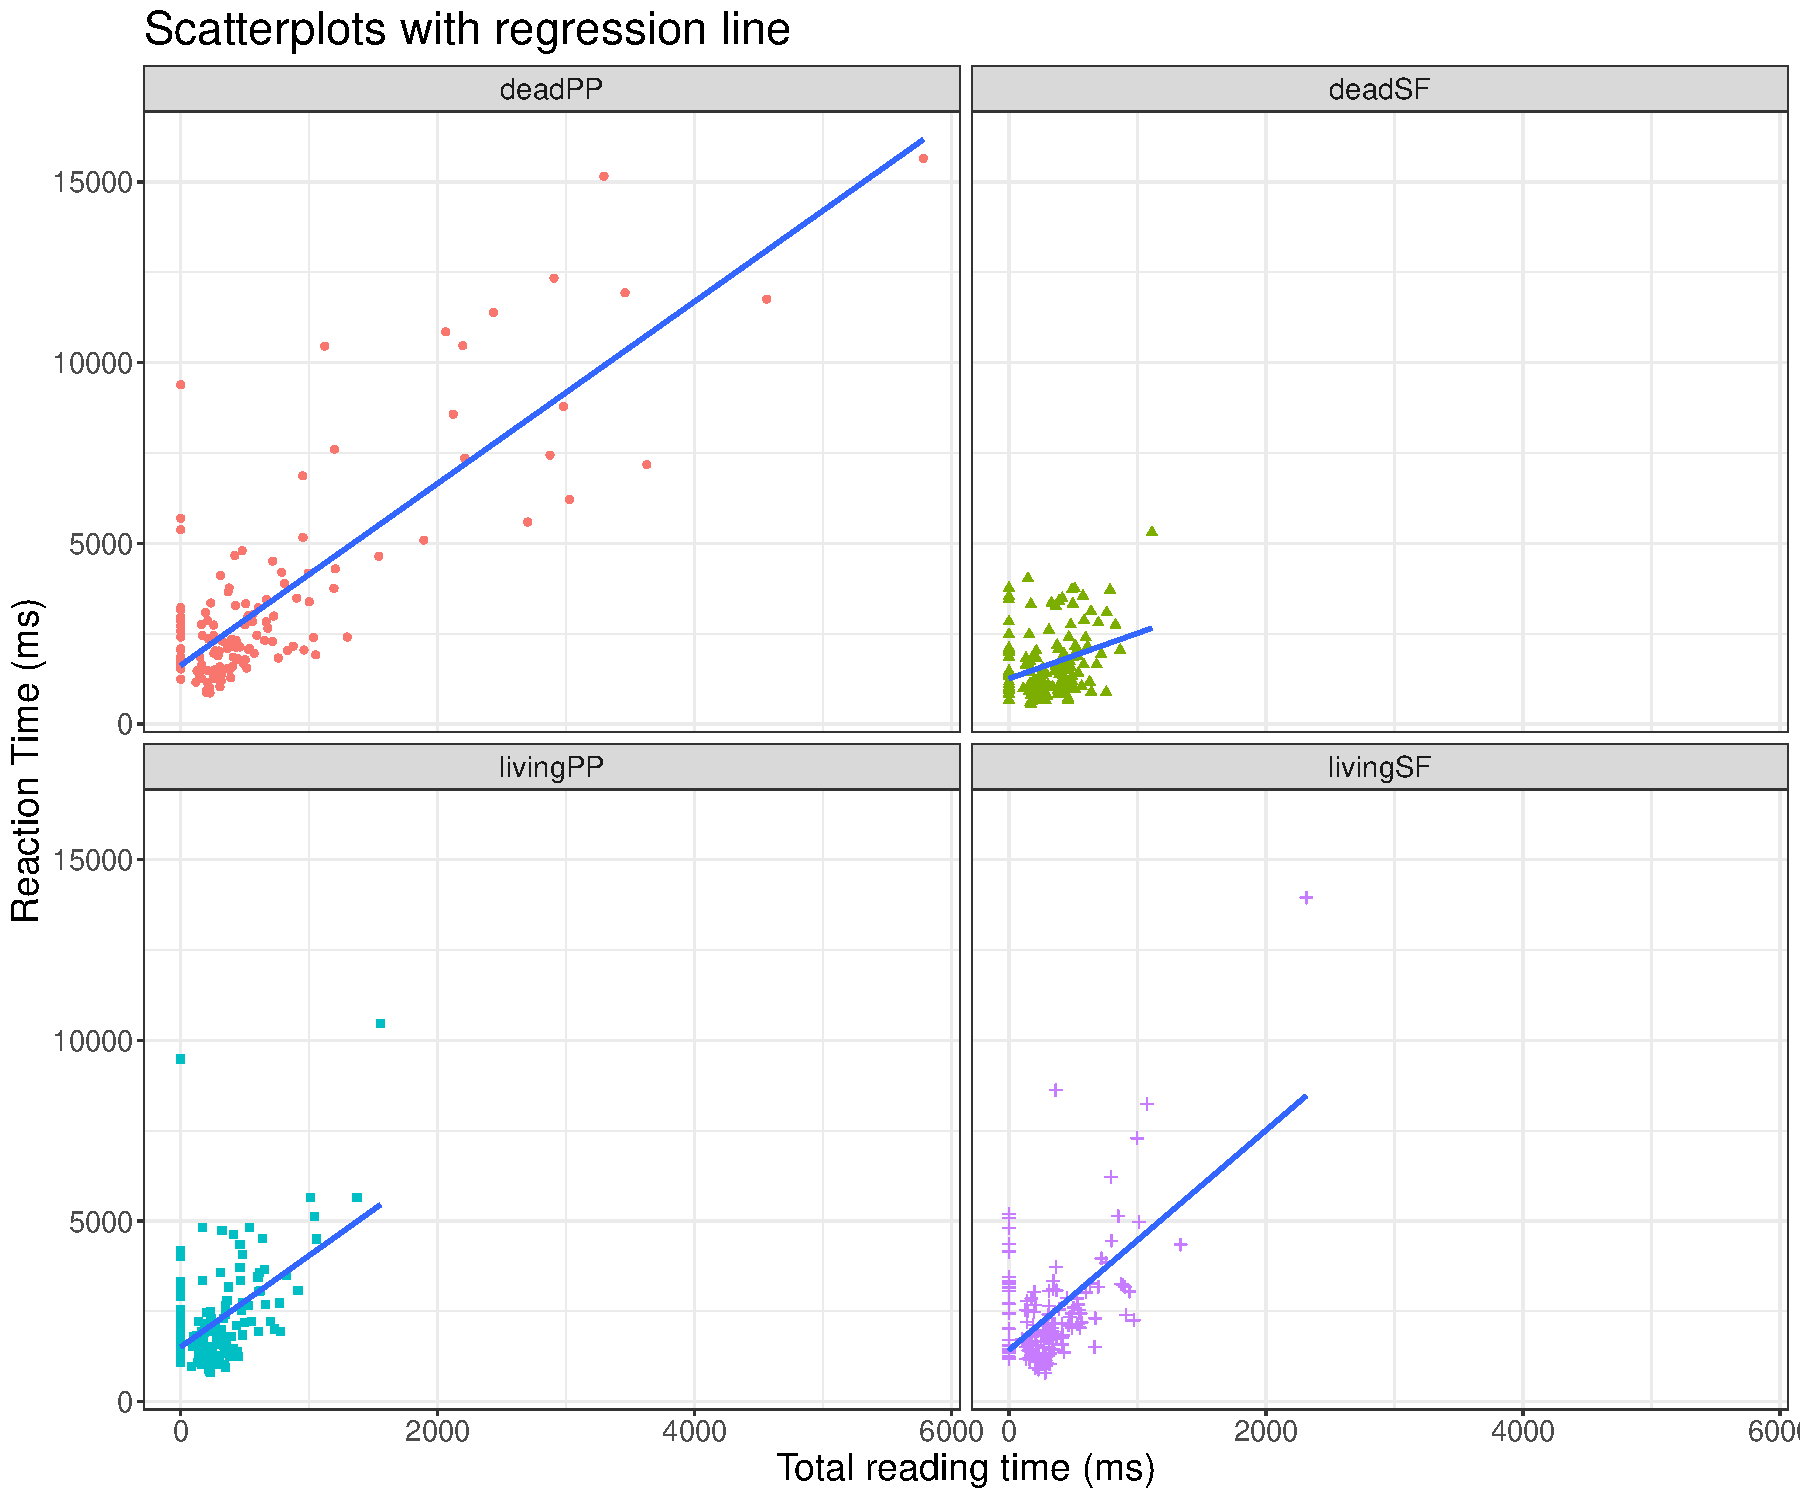
\includegraphics{_lin_reg1_files/figure-pdf/unnamed-chunk-6-1.pdf}

}

\end{figure}

\hypertarget{slopes-b_1}{%
\subsection{\texorpdfstring{Slopes
(\(b_1\))}{Slopes (b\_1)}}\label{slopes-b_1}}

\begin{itemize}
\tightlist
\item
  slopes describe a change in \(x\) (\(\Delta x\)) over a change in
  \(y\) (\(\Delta y\))

  \begin{itemize}
  \tightlist
  \item
    positive slope: as \(x\) increases, \(y\) increases
  \item
    negative slope: as \(x\) increases, \(y\) decreases
  \item
    if the slope is 0, there is no change in \(y\) as a function of
    \(x\)
  \end{itemize}
\end{itemize}

\[
slope = \frac{\Delta x}{\Delta y}
\]

\begin{itemize}
\tightlist
\item
  or: the change in \(y\) when \(x\) increase by 1 unit

  \begin{itemize}
  \tightlist
  \item
    sometimes referred to as ``rise over run'': how do you `rise' in
    \(y\) for a given `run' in \(x\)?
  \end{itemize}
\end{itemize}

\hypertarget{slopes-b_1-1}{%
\subsection*{\texorpdfstring{Slopes
(\(b_1\))}{Slopes (b\_1)}}\label{slopes-b_1-1}}
\addcontentsline{toc}{subsection}{Slopes (\(b_1\))}

\hypertarget{intercepts-b_0}{%
\subsection{\texorpdfstring{Intercepts
(\(b_0\))}{Intercepts (b\_0)}}\label{intercepts-b_0}}

\hypertarget{varying-slopes-and-intercepts}{%
\subsection{Varying slopes and
intercepts}\label{varying-slopes-and-intercepts}}

\begin{figure}

{\centering 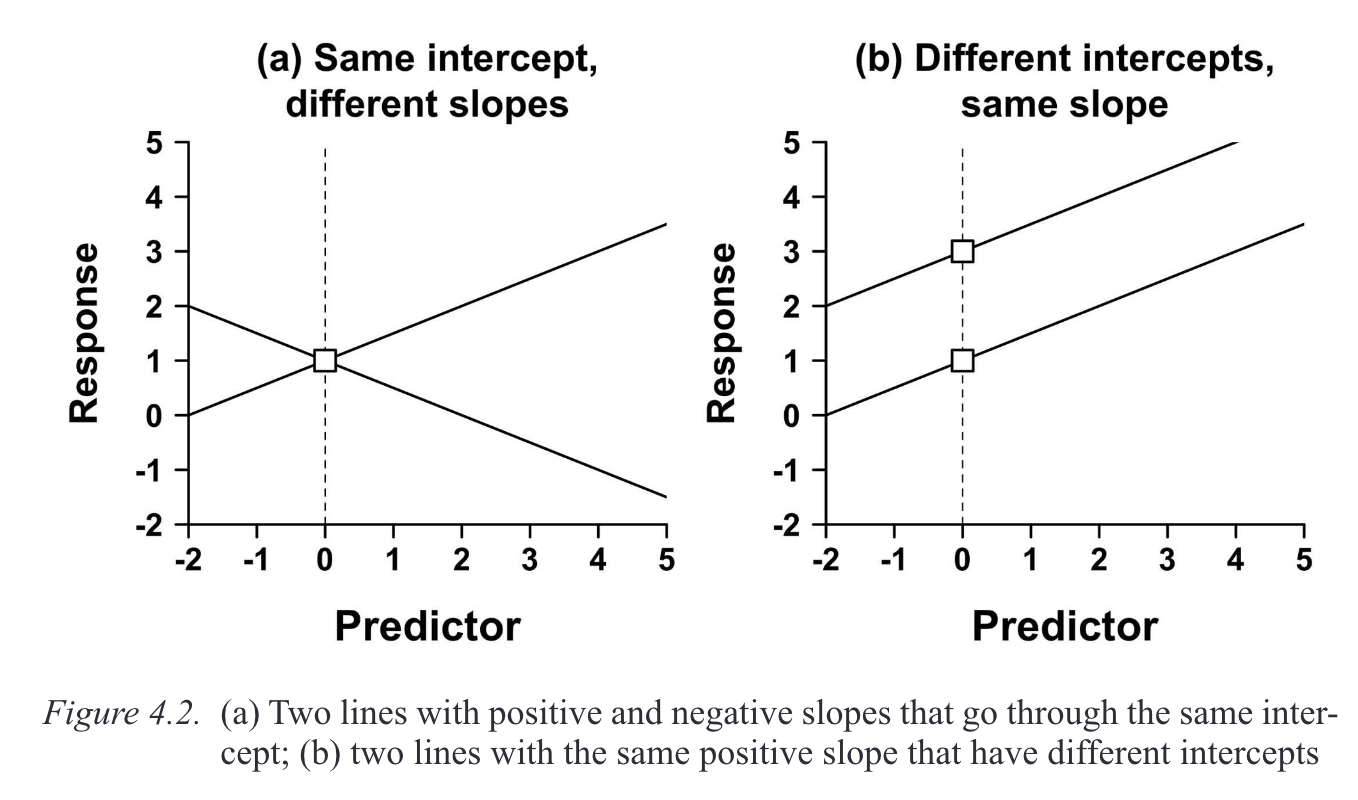
\includegraphics[width=4.53in,height=\textheight]{_lin_reg1_files/figure-pdf/unnamed-chunk-8-1.png}

}

\caption{Image source: Winter (2019) (all rights reserved)}

\end{figure}

\hypertarget{linear-regression-first-fixation-duration}{%
\section{Linear regression: first fixation
duration}\label{linear-regression-first-fixation-duration}}

\hypertarget{first-fixation-time}{%
\subsection{First-fixation time}\label{first-fixation-time}}

\begin{Shaded}
\begin{Highlighting}[]
\NormalTok{fit\_ff\_b0 }\OtherTok{\textless{}{-}}\NormalTok{ df\_crit\_verb }\SpecialCharTok{\%\textgreater{}\%}
  \FunctionTok{lm}\NormalTok{(ff }\SpecialCharTok{\textasciitilde{}} \DecValTok{1}\NormalTok{, }\AttributeTok{data =}\NormalTok{ .)}
\end{Highlighting}
\end{Shaded}

\begin{itemize}
\tightlist
\item
  \texttt{lm()} function formula syntax can be read as: ff predicted by
  the intercept (\texttt{1} is a placeholder for the intercept)

  \begin{itemize}
  \tightlist
  \item
    the intercept is included by default
  \item
    if you omit the \texttt{1}, the intercept is still included in the
    formula
  \item
    if you wanted to remove the intercept (which you often don't), you
    could replace \texttt{1} with \texttt{0}
  \end{itemize}
\end{itemize}

\hypertarget{summary}{%
\subsubsection{Summary}\label{summary}}

\begin{Shaded}
\begin{Highlighting}[]
\FunctionTok{summary}\NormalTok{(fit\_ff\_b0)}
\end{Highlighting}
\end{Shaded}

\begin{verbatim}

Call:
lm(formula = ff ~ 1, data = .)

Residuals:
    Min      1Q  Median      3Q     Max 
-166.59  -27.09   10.41   50.41  294.42 

Coefficients:
            Estimate Std. Error t value            Pr(>|t|)    
(Intercept)  166.585      3.847    43.3 <0.0000000000000002 ***
---
Signif. codes:  0 '***' 0.001 '**' 0.01 '*' 0.05 '.' 0.1 ' ' 1

Residual standard error: 90.95 on 558 degrees of freedom
\end{verbatim}

\hypertarget{annotated-cell-8}{%
\label{annotated-cell-8}}%
\begin{Shaded}
\begin{Highlighting}[]
\NormalTok{Call}\SpecialCharTok{:}
\FunctionTok{lm}\NormalTok{(}\AttributeTok{formula =}\NormalTok{ ff }\SpecialCharTok{\textasciitilde{}} \DecValTok{1}\NormalTok{, }\AttributeTok{data =}\NormalTok{ .) }\CommentTok{\#\textless{}1\textgreater{}}

\NormalTok{Residuals}\SpecialCharTok{:}
\NormalTok{     Min       1Q   Median       3Q      Max }
\SpecialCharTok{{-}}\FloatTok{193.395}  \SpecialCharTok{{-}}\FloatTok{34.395}   \SpecialCharTok{{-}}\FloatTok{8.395}   \FloatTok{30.605}  \FloatTok{267.605}  \CommentTok{\#\textless{}2\textgreater{}}

\NormalTok{Coefficients}\SpecialCharTok{:}
\NormalTok{            Estimate Std. Error t value            }\FunctionTok{Pr}\NormalTok{(}\SpecialCharTok{\textgreater{}}\ErrorTok{|}\NormalTok{t}\SpecialCharTok{|}\NormalTok{)    }\CommentTok{\#\textless{}3\textgreater{}}
\NormalTok{(Intercept)  }\FloatTok{193.395}      \FloatTok{2.777}   \FloatTok{69.63} \SpecialCharTok{\textless{}}\FloatTok{0.0000000000000002} \SpecialCharTok{**}\ErrorTok{*} \CommentTok{\#\textless{}4\textgreater{}}
\SpecialCharTok{{-}{-}{-}}
\NormalTok{Signif. codes}\SpecialCharTok{:}  \DecValTok{0}\NormalTok{ ‘}\SpecialCharTok{**}\ErrorTok{*}\NormalTok{’ }\FloatTok{0.001}\NormalTok{ ‘}\SpecialCharTok{**}\NormalTok{’ }\FloatTok{0.01}\NormalTok{ ‘}\SpecialCharTok{*}\NormalTok{’ }\FloatTok{0.05}\NormalTok{ ‘.’ }\FloatTok{0.1}\NormalTok{ ‘ ’ }\DecValTok{1} \CommentTok{\#\textless{}5\textgreater{}}

\NormalTok{Residual standard error}\SpecialCharTok{:} \FloatTok{65.66}\NormalTok{ on }\DecValTok{558}\NormalTok{ degrees of freedom }\CommentTok{\#\textless{}6\textgreater{}}
\end{Highlighting}
\end{Shaded}

\begin{description}
\tightlist
\item[\circled{1}]
formula repetition
\item[\circled{2}]
residuals: differences between observed values and those predicted by
the model
\item[\circled{3}]
names for columns Estimates, standard error, t-value, p-value
(\texttt{Pr(\textgreater{}\textbar{}t\textbar{})})
\item[\circled{4}]
Intercept (\(b_0\)), i.e., value of \(y\) (first fix.) with a move of
one unit of \(x\) (lifetime)
\item[\circled{5}]
R\(^2\), a measure of model fit (squared residuals); percentage of
variance in the data shared with the predictor (higher numbers are
better\ldots this is pretty low)
\end{description}

\begin{itemize}
\tightlist
\item
  Adjusted R\(^2\) takes into account the number of predictors. The more
  fixed effects, the lower Adjusted R\(^2\) will be.
\end{itemize}

\begin{enumerate}
\def\labelenumi{\arabic{enumi})}
\setcounter{enumi}{6}
\tightlist
\item
  Output from an ANOVA
\end{enumerate}

\hypertarget{first-fixation-duration-and-lifetime}{%
\subsection{First-fixation duration and
lifetime}\label{first-fixation-duration-and-lifetime}}

\begin{itemize}
\tightlist
\item
  let's stick to first-fixation time,
\end{itemize}

\hypertarget{method-of-least-squares}{%
\subsection{Method of least squares}\label{method-of-least-squares}}

\begin{itemize}
\tightlist
\item
  first, order our predictor

  \begin{itemize}
  \tightlist
  \item
    we predict longer reading times for dead versus living, so order
    living dead
  \end{itemize}
\end{itemize}

\begin{Shaded}
\begin{Highlighting}[]
\CommentTok{\# order factor levels}
\NormalTok{df\_crit\_verb}\SpecialCharTok{$}\NormalTok{lifetime }\OtherTok{\textless{}{-}} \FunctionTok{factor}\NormalTok{(df\_crit\_verb}\SpecialCharTok{$}\NormalTok{lifetime, }\AttributeTok{levels =} \FunctionTok{c}\NormalTok{(}\StringTok{"living"}\NormalTok{,}\StringTok{"dead"}\NormalTok{))}

\CommentTok{\# set contrasts}
\FunctionTok{contrasts}\NormalTok{(df\_crit\_verb}\SpecialCharTok{$}\NormalTok{lifetime) }\OtherTok{\textless{}{-}} \FunctionTok{c}\NormalTok{(}\SpecialCharTok{{-}}\FloatTok{0.5}\NormalTok{,}\SpecialCharTok{+}\FloatTok{0.5}\NormalTok{); }\FunctionTok{contrasts}\NormalTok{(df\_crit\_verb}\SpecialCharTok{$}\NormalTok{lifetime)}
\end{Highlighting}
\end{Shaded}

\begin{verbatim}
       [,1]
living -0.5
dead    0.5
\end{verbatim}

\hypertarget{fit-model}{%
\subsection{fit model}\label{fit-model}}

\begin{itemize}
\tightlist
\item
  let's exclude missing observations (0)
\end{itemize}

\begin{Shaded}
\begin{Highlighting}[]
\CommentTok{\# fit simple linear model}
\NormalTok{fit\_ff }\OtherTok{\textless{}{-}}\NormalTok{ df\_crit\_verb }\SpecialCharTok{\%\textgreater{}\%}
  \FunctionTok{filter}\NormalTok{(ff }\SpecialCharTok{\textgreater{}} \DecValTok{0}\NormalTok{) }\SpecialCharTok{\%\textgreater{}\%}
  \FunctionTok{lm}\NormalTok{(ff }\SpecialCharTok{\textasciitilde{}}\NormalTok{ lifetime, }\AttributeTok{data =}\NormalTok{ .)}
\end{Highlighting}
\end{Shaded}

\begin{Shaded}
\begin{Highlighting}[]
\CommentTok{\# alternatively}
\NormalTok{fit\_ff }\OtherTok{\textless{}{-}} \FunctionTok{lm}\NormalTok{(ff }\SpecialCharTok{\textasciitilde{}}\NormalTok{ lifetime, }
            \AttributeTok{data =}\NormalTok{ df\_crit\_verb, }\AttributeTok{subset =}\NormalTok{ ff }\SpecialCharTok{\textgreater{}} \DecValTok{0}\NormalTok{)}
\end{Highlighting}
\end{Shaded}

\hypertarget{coefficients-table-with-summary}{%
\subsection{\texorpdfstring{Coefficients table with
\texttt{summary()}}{Coefficients table with summary()}}\label{coefficients-table-with-summary}}

\hypertarget{annotated-cell-1}{%
\label{annotated-cell-1}}%
\begin{Shaded}
\begin{Highlighting}[]
\SpecialCharTok{\textgreater{}} \FunctionTok{summary}\NormalTok{(fit\_ff)}

\NormalTok{Call}\SpecialCharTok{:}
\FunctionTok{lm}\NormalTok{(}\AttributeTok{formula =}\NormalTok{ ff }\SpecialCharTok{\textasciitilde{}}\NormalTok{ lifetime, }\AttributeTok{data =}\NormalTok{ df\_crit\_verb, }\AttributeTok{subset =}\NormalTok{ ff }\SpecialCharTok{\textgreater{}} \DecValTok{0}\NormalTok{) }\CommentTok{\#\textless{}1\textgreater{}}

\NormalTok{Residuals}\SpecialCharTok{:}                                                        \CommentTok{\#\textless{}2\textgreater{}}
\NormalTok{    Min      1Q  Median      3Q     Max }
\SpecialCharTok{{-}}\FloatTok{118.78}  \SpecialCharTok{{-}}\FloatTok{37.78}  \SpecialCharTok{{-}}\FloatTok{11.39}   \FloatTok{25.22}  \FloatTok{264.61} 

\NormalTok{Coefficients}\SpecialCharTok{:}
\NormalTok{             Estimate Std. Error t value }\FunctionTok{Pr}\NormalTok{(}\SpecialCharTok{\textgreater{}}\ErrorTok{|}\NormalTok{t}\SpecialCharTok{|}\NormalTok{)                }\CommentTok{\#\textless{}3\textgreater{}}
\NormalTok{(Intercept)   }\FloatTok{199.089}      \FloatTok{2.466}  \FloatTok{80.743}   \SpecialCharTok{\textless{}}\FloatTok{2e{-}16} \SpecialCharTok{**}\ErrorTok{*}            \CommentTok{\#\textless{}4\textgreater{}}
\NormalTok{lifetimedead    }\FloatTok{5.388}      \FloatTok{4.931}   \FloatTok{1.093}    \FloatTok{0.275}                \CommentTok{\#\textless{}5\textgreater{}}
\SpecialCharTok{{-}{-}{-}}
\NormalTok{Signif. codes}\SpecialCharTok{:}  \DecValTok{0}\NormalTok{ ‘}\SpecialCharTok{**}\ErrorTok{*}\NormalTok{’ }\FloatTok{0.001}\NormalTok{ ‘}\SpecialCharTok{**}\NormalTok{’ }\FloatTok{0.01}\NormalTok{ ‘}\SpecialCharTok{*}\NormalTok{’ }\FloatTok{0.05}\NormalTok{ ‘.’ }\FloatTok{0.1}\NormalTok{ ‘ ’ }\DecValTok{1}

\NormalTok{Residual standard error}\SpecialCharTok{:} \FloatTok{57.46}\NormalTok{ on }\DecValTok{541}\NormalTok{ degrees of freedom}
\NormalTok{Multiple R}\SpecialCharTok{{-}}\NormalTok{squared}\SpecialCharTok{:}  \FloatTok{0.002202}\NormalTok{,  Adjusted R}\SpecialCharTok{{-}}\NormalTok{squared}\SpecialCharTok{:}  \FloatTok{0.0003575}   \CommentTok{\#\textless{}6\textgreater{}}
\NormalTok{F}\SpecialCharTok{{-}}\NormalTok{statistic}\SpecialCharTok{:} \FloatTok{1.194}\NormalTok{ on }\DecValTok{1}\NormalTok{ and }\DecValTok{541}\NormalTok{ DF,  p}\SpecialCharTok{{-}}\NormalTok{value}\SpecialCharTok{:} \FloatTok{0.275}              \CommentTok{\#\textless{}7\textgreater{}}
\end{Highlighting}
\end{Shaded}

\begin{description}
\tightlist
\item[\circled{1}]
formula
\item[\circled{2}]
Residuals: differences between observed values and those predicted by
the model
\item[\circled{3}]
Names for columns Estimates, SE, t-value, p-value
\item[\circled{4}]
Intercept (\(b_0\)), i.e., value of \(y\) (first fix.) with a move of
one unit of \(x\) (lifetime)
\item[\circled{5}]
Slope (\(b_1\)), i.e., change in first fixation going from \texttt{dead}
to \texttt{living}
\item[\circled{6}]
Output from an ANOVA
\end{description}

\begin{itemize}
\tightlist
\item
  what is the \textbf{intercept}?
\item
  is the \textbf{slope} positive or negative?

  \begin{itemize}
  \tightlist
  \item
    what is it's value?
  \end{itemize}
\item
  this is what the slope would look like:
\end{itemize}

\hypertarget{understanding-the-summary}{%
\subsubsection{Understanding the
summary}\label{understanding-the-summary}}

\begin{itemize}
\tightlist
\item
  let's compute summary statistics based on \emph{lifetime}

  \begin{itemize}
  \tightlist
  \item
    then compare this to the model output
  \end{itemize}
\end{itemize}

\ul{Exercises}

\begin{enumerate}
\def\labelenumi{\arabic{enumi}.}
\tightlist
\item
  Subtract the mean first-fixation reading time of \texttt{dead} from
  that of \texttt{living}

  \begin{itemize}
  \tightlist
  \item
    what does this correspond to in the model summary?
  \end{itemize}
\item
  Compute the mean of \texttt{dead}+\texttt{living}

  \begin{itemize}
  \tightlist
  \item
    what does this correspond to in the model summary?
  \end{itemize}
\item
  Divide the slope in 2. Subtract this from the mean of \texttt{dead}.

  \begin{itemize}
  \tightlist
  \item
    what does this correspond to?
  \end{itemize}
\end{enumerate}

\ul{Summary statistics}

\begin{Shaded}
\begin{Highlighting}[]
\CommentTok{\# compute summary }
\NormalTok{summary\_ff\_life }\OtherTok{\textless{}{-}}\NormalTok{ df\_crit\_verb }\SpecialCharTok{|\textgreater{}} 
  \FunctionTok{filter}\NormalTok{(region}\SpecialCharTok{==}\StringTok{"verb"}\NormalTok{,}
\NormalTok{         ff }\SpecialCharTok{\textgreater{}} \DecValTok{0}\NormalTok{) }\SpecialCharTok{|\textgreater{}} 
  \FunctionTok{group\_by}\NormalTok{(lifetime) }\SpecialCharTok{\%\textgreater{}\%}
  \FunctionTok{summarise}\NormalTok{(}\AttributeTok{N =} \FunctionTok{n}\NormalTok{(),}
            \AttributeTok{mean =} \FunctionTok{mean}\NormalTok{(ff, }\AttributeTok{na.rm =}\NormalTok{ T),}
            \AttributeTok{sd =} \FunctionTok{sd}\NormalTok{(ff, }\AttributeTok{na.rm =}\NormalTok{ T)) }\SpecialCharTok{\%\textgreater{}\%}
  \CommentTok{\# compute standard error, confidence intervals, and lower/upper ci bounds}
  \FunctionTok{mutate}\NormalTok{(}\AttributeTok{se =}\NormalTok{ sd }\SpecialCharTok{/} \FunctionTok{sqrt}\NormalTok{(N),}
         \AttributeTok{ci =} \FunctionTok{qt}\NormalTok{(}\DecValTok{1} \SpecialCharTok{{-}}\NormalTok{ (}\FloatTok{0.05} \SpecialCharTok{/} \DecValTok{2}\NormalTok{), N }\SpecialCharTok{{-}} \DecValTok{1}\NormalTok{) }\SpecialCharTok{*}\NormalTok{ se,}
         \AttributeTok{lower.ci =}\NormalTok{ mean }\SpecialCharTok{{-}} \FunctionTok{qt}\NormalTok{(}\DecValTok{1} \SpecialCharTok{{-}}\NormalTok{ (}\FloatTok{0.05} \SpecialCharTok{/} \DecValTok{2}\NormalTok{), N }\SpecialCharTok{{-}} \DecValTok{1}\NormalTok{) }\SpecialCharTok{*}\NormalTok{ se,}
         \AttributeTok{upper.ci =}\NormalTok{ mean }\SpecialCharTok{+} \FunctionTok{qt}\NormalTok{(}\DecValTok{1} \SpecialCharTok{{-}}\NormalTok{ (}\FloatTok{0.05} \SpecialCharTok{/} \DecValTok{2}\NormalTok{), N }\SpecialCharTok{{-}} \DecValTok{1}\NormalTok{) }\SpecialCharTok{*}\NormalTok{ se)}

\NormalTok{knitr}\SpecialCharTok{::}\FunctionTok{kable}\NormalTok{(summary\_ff\_life, }\AttributeTok{digits=}\DecValTok{3}\NormalTok{,}
             \AttributeTok{caption =} \StringTok{"Summmary statistics for first{-}fixation duration at the verb region"}\NormalTok{) }\SpecialCharTok{\%\textgreater{}\%} 
\NormalTok{  kableExtra}\SpecialCharTok{::}\FunctionTok{kable\_styling}\NormalTok{(}\AttributeTok{font\_size =} \DecValTok{24}\NormalTok{,}
                            \AttributeTok{position =} \StringTok{"left"}\NormalTok{)}
\end{Highlighting}
\end{Shaded}

\begin{table}

\caption{Summmary statistics for first-fixation duration at the verb region}
\fontsize{24}{26}\selectfont
\begin{tabular}[t]{l|r|r|r|r|r|r|r}
\hline
lifetime & N & mean & sd & se & ci & lower.ci & upper.ci\\
\hline
living & 232 & 197.927 & 59.581 & 3.912 & 7.707 & 190.220 & 205.634\\
\hline
dead & 234 & 201.718 & 54.751 & 3.579 & 7.052 & 194.666 & 208.770\\
\hline
\end{tabular}
\end{table}

\ul{Model summary}

\begin{Shaded}
\begin{Highlighting}[]
\FunctionTok{summary}\NormalTok{(fit\_ff)}
\end{Highlighting}
\end{Shaded}

\begin{verbatim}

Call:
lm(formula = ff ~ lifetime, data = df_crit_verb, subset = ff > 
    0)

Residuals:
    Min      1Q  Median      3Q     Max 
-118.72  -35.52  -10.72   25.23  263.07 

Coefficients:
            Estimate Std. Error t value            Pr(>|t|)    
(Intercept)  199.822      2.650  75.403 <0.0000000000000002 ***
lifetime1      3.791      5.300   0.715               0.475    
---
Signif. codes:  0 '***' 0.001 '**' 0.01 '*' 0.05 '.' 0.1 ' ' 1

Residual standard error: 57.21 on 464 degrees of freedom
Multiple R-squared:  0.001102,  Adjusted R-squared:  -0.001051 
F-statistic: 0.5117 on 1 and 464 DF,  p-value: 0.4748
\end{verbatim}

\hypertarget{section}{%
\subsection*{}\label{section}}
\addcontentsline{toc}{subsection}{}

\begin{tcolorbox}[enhanced jigsaw, leftrule=.75mm, bottomrule=.15mm, breakable, left=2mm, colback=white, bottomtitle=1mm, colbacktitle=quarto-callout-tip-color!10!white, opacitybacktitle=0.6, titlerule=0mm, colframe=quarto-callout-tip-color-frame, toprule=.15mm, rightrule=.15mm, arc=.35mm, opacityback=0, toptitle=1mm, title=\textcolor{quarto-callout-tip-color}{\faLightbulb}\hspace{0.5em}{\texttt{broom} package for tidy model summaries}, coltitle=black]

\begin{Shaded}
\begin{Highlighting}[]
\CommentTok{\# install.packages("broom")}
\FunctionTok{library}\NormalTok{(broom)}
\FunctionTok{tidy}\NormalTok{(fit\_ff)}
\end{Highlighting}
\end{Shaded}

\begin{verbatim}
# A tibble: 2 x 5
  term        estimate std.error statistic   p.value
  <chr>          <dbl>     <dbl>     <dbl>     <dbl>
1 (Intercept)   200.        2.65    75.4   1.61e-262
2 lifetime1       3.79      5.30     0.715 4.75e-  1
\end{verbatim}

\begin{Shaded}
\begin{Highlighting}[]
\FunctionTok{glance}\NormalTok{(fit\_ff)}
\end{Highlighting}
\end{Shaded}

\begin{verbatim}
# A tibble: 1 x 12
  r.squared adj.r.squared sigma statistic p.value    df logLik   AIC   BIC
      <dbl>         <dbl> <dbl>     <dbl>   <dbl> <dbl>  <dbl> <dbl> <dbl>
1   0.00110      -0.00105  57.2     0.512   0.475     1 -2546. 5098. 5110.
# i 3 more variables: deviance <dbl>, df.residual <int>, nobs <int>
\end{verbatim}

\begin{Shaded}
\begin{Highlighting}[]
\NormalTok{df\_crit\_verb }\SpecialCharTok{\%\textgreater{}\%}
  \CommentTok{\# mutate(life\_c = if\_else(lifetime=="living",{-}0.5,+0.5)) \%\textgreater{}\%}
  \FunctionTok{select}\NormalTok{(ff,fp,rpd,tt) }\SpecialCharTok{\%\textgreater{}\%}
  \FunctionTok{cor}\NormalTok{()}
\end{Highlighting}
\end{Shaded}

\begin{verbatim}
           ff        fp       rpd        tt
ff  1.0000000 0.7024805 0.6751225 0.3107962
fp  0.7024805 1.0000000 0.9303347 0.4528066
rpd 0.6751225 0.9303347 1.0000000 0.4317107
tt  0.3107962 0.4528066 0.4317107 1.0000000
\end{verbatim}

\begin{Shaded}
\begin{Highlighting}[]
\CommentTok{\# fit simple linear model with log}
\NormalTok{fit\_ff\_log }\OtherTok{\textless{}{-}}\NormalTok{ df\_crit\_verb }\SpecialCharTok{\%\textgreater{}\%}
  \FunctionTok{filter}\NormalTok{(ff }\SpecialCharTok{\textgreater{}} \DecValTok{0}\NormalTok{) }\SpecialCharTok{\%\textgreater{}\%} \CommentTok{\# because you can\textquotesingle{}t log transform 0}
  \FunctionTok{mutate}\NormalTok{(}\AttributeTok{ff\_c =}\NormalTok{ ff}\SpecialCharTok{{-}}\FunctionTok{mean}\NormalTok{(ff)) }\SpecialCharTok{\%\textgreater{}\%}
  \FunctionTok{lm}\NormalTok{(ff\_c }\SpecialCharTok{\textasciitilde{}}\NormalTok{ lifetime, }\AttributeTok{data =}\NormalTok{ .)}
\FunctionTok{summary}\NormalTok{(fit\_ff\_log)}
\end{Highlighting}
\end{Shaded}

\begin{verbatim}

Call:
lm(formula = ff_c ~ lifetime, data = .)

Residuals:
    Min      1Q  Median      3Q     Max 
-118.72  -35.52  -10.72   25.23  263.07 

Coefficients:
             Estimate Std. Error t value Pr(>|t|)
(Intercept) -0.008136   2.650072  -0.003    0.998
lifetime1    3.791225   5.300143   0.715    0.475

Residual standard error: 57.21 on 464 degrees of freedom
Multiple R-squared:  0.001102,  Adjusted R-squared:  -0.001051 
F-statistic: 0.5117 on 1 and 464 DF,  p-value: 0.4748
\end{verbatim}

\end{tcolorbox}

\hypertarget{exploring-the-model}{%
\subsection{Exploring the model}\label{exploring-the-model}}

\begin{itemize}
\tightlist
\item
  the linear model contains \emph{fitted} values corresponding to our
  \emph{observed} values

  \begin{itemize}
  \tightlist
  \item
    these \emph{fitted} values are fit to a straight line
  \item
    our \emph{observed} values are not fit to a straight line
  \item
    the \emph{residuals} are the differences along the \(y\) axis from
    the fitted to the observed values
  \end{itemize}
\end{itemize}

\hypertarget{exploring-the-model-1}{%
\subsection*{Exploring the model}\label{exploring-the-model-1}}
\addcontentsline{toc}{subsection}{Exploring the model}

\begin{Shaded}
\begin{Highlighting}[]
\CommentTok{\# how many observed values did we enter into the model?}
\NormalTok{df\_crit\_verb }\SpecialCharTok{|\textgreater{}} 
  \FunctionTok{filter}\NormalTok{(ff }\SpecialCharTok{\textgreater{}} \DecValTok{0}\NormalTok{) }\SpecialCharTok{|\textgreater{}} 
  \FunctionTok{nrow}\NormalTok{()}
\end{Highlighting}
\end{Shaded}

\begin{verbatim}
[1] 466
\end{verbatim}

\begin{Shaded}
\begin{Highlighting}[]
\CommentTok{\# how many observed values did we enter into the model?}
\FunctionTok{length}\NormalTok{(}\FunctionTok{fitted}\NormalTok{(fit\_ff))}
\end{Highlighting}
\end{Shaded}

\begin{verbatim}
[1] 466
\end{verbatim}

\hypertarget{exploring-the-model-2}{%
\subsection*{Exploring the model}\label{exploring-the-model-2}}
\addcontentsline{toc}{subsection}{Exploring the model}

\begin{Shaded}
\begin{Highlighting}[]
\CommentTok{\# how many observed values did we enter into the model?}
\FunctionTok{head}\NormalTok{(}\FunctionTok{fitted}\NormalTok{(fit\_ff))}
\end{Highlighting}
\end{Shaded}

\begin{verbatim}
      81       82       83       84       85       86 
197.9267 197.9267 201.7179 197.9267 201.7179 197.9267 
\end{verbatim}

\begin{Shaded}
\begin{Highlighting}[]
\CommentTok{\# how many observed values did we enter into the model?}
\FunctionTok{head}\NormalTok{(df\_crit\_verb}\SpecialCharTok{$}\NormalTok{ff)}
\end{Highlighting}
\end{Shaded}

\begin{verbatim}
[1] 0 0 0 0 0 0
\end{verbatim}

\begin{Shaded}
\begin{Highlighting}[]
\FunctionTok{head}\NormalTok{(}\FunctionTok{fitted}\NormalTok{(fit\_ff)) }\SpecialCharTok{{-}} \FunctionTok{head}\NormalTok{(df\_crit\_verb}\SpecialCharTok{$}\NormalTok{ff)}
\end{Highlighting}
\end{Shaded}

\begin{verbatim}
      81       82       83       84       85       86 
197.9267 197.9267 201.7179 197.9267 201.7179 197.9267 
\end{verbatim}

\begin{Shaded}
\begin{Highlighting}[]
\CommentTok{\# look at the residuals}
\FunctionTok{head}\NormalTok{(}\FunctionTok{residuals}\NormalTok{(fit\_ff))}
\end{Highlighting}
\end{Shaded}

\begin{verbatim}
        81         82         83         84         85         86 
-22.926724   9.073276  26.282051  33.073276  10.282051 -29.926724 
\end{verbatim}

\hypertarget{exploring-the-model-3}{%
\subsection*{Exploring the model}\label{exploring-the-model-3}}
\addcontentsline{toc}{subsection}{Exploring the model}

\begin{Shaded}
\begin{Highlighting}[]
\FunctionTok{coef}\NormalTok{(fit\_ff)}
\end{Highlighting}
\end{Shaded}

\begin{verbatim}
(Intercept)   lifetime1 
 199.822336    3.791225 
\end{verbatim}

\begin{Shaded}
\begin{Highlighting}[]
\FunctionTok{coef}\NormalTok{(fit\_ff)[}\StringTok{\textquotesingle{}(Intercept)\textquotesingle{}}\NormalTok{] }\SpecialCharTok{+} \FunctionTok{coef}\NormalTok{(fit\_ff)[}\StringTok{\textquotesingle{}lifetime1\textquotesingle{}}\NormalTok{] }\SpecialCharTok{*} \SpecialCharTok{{-}}\FloatTok{0.5}
\end{Highlighting}
\end{Shaded}

\begin{verbatim}
(Intercept) 
   197.9267 
\end{verbatim}

\begin{Shaded}
\begin{Highlighting}[]
\FunctionTok{coef}\NormalTok{(fit\_ff)[}\StringTok{\textquotesingle{}(Intercept)\textquotesingle{}}\NormalTok{] }\SpecialCharTok{+} \FunctionTok{coef}\NormalTok{(fit\_ff)[}\StringTok{\textquotesingle{}lifetime1\textquotesingle{}}\NormalTok{] }\SpecialCharTok{*} \FloatTok{0.5}
\end{Highlighting}
\end{Shaded}

\begin{verbatim}
(Intercept) 
   201.7179 
\end{verbatim}

\hypertarget{assumptions}{%
\subsection{Assumptions}\label{assumptions}}

\begin{itemize}
\tightlist
\item
  normality assumption

  \begin{itemize}
  \tightlist
  \item
    residuals of the model are (approximately) normally distributed
  \end{itemize}
\item
  constant variance assumption (homoscedasticity)

  \begin{itemize}
  \tightlist
  \item
    spread of residuals should be (approximately) equal along the
    regression line
  \end{itemize}
\end{itemize}

\hypertarget{normality-assumption}{%
\subsubsection{Normality assumption}\label{normality-assumption}}

\begin{Shaded}
\begin{Highlighting}[]
\NormalTok{df\_crit\_verb }\SpecialCharTok{|\textgreater{}} 
  \FunctionTok{filter}\NormalTok{(ff }\SpecialCharTok{\textgreater{}} \DecValTok{0}\NormalTok{) }\SpecialCharTok{|\textgreater{}} 
  \FunctionTok{mutate}\NormalTok{(}\AttributeTok{half =} \FunctionTok{if\_else}\NormalTok{(trial }\SpecialCharTok{\textgreater{}=} \DecValTok{104}\NormalTok{, }\StringTok{"1st"}\NormalTok{,}\StringTok{"2nd"}\NormalTok{)) }\SpecialCharTok{|\textgreater{}} 
\NormalTok{  ggpubr}\SpecialCharTok{::}\FunctionTok{ggqqplot}\NormalTok{(}\AttributeTok{x =} \StringTok{"ff"}\NormalTok{)}
\end{Highlighting}
\end{Shaded}

\begin{figure}[H]

{\centering 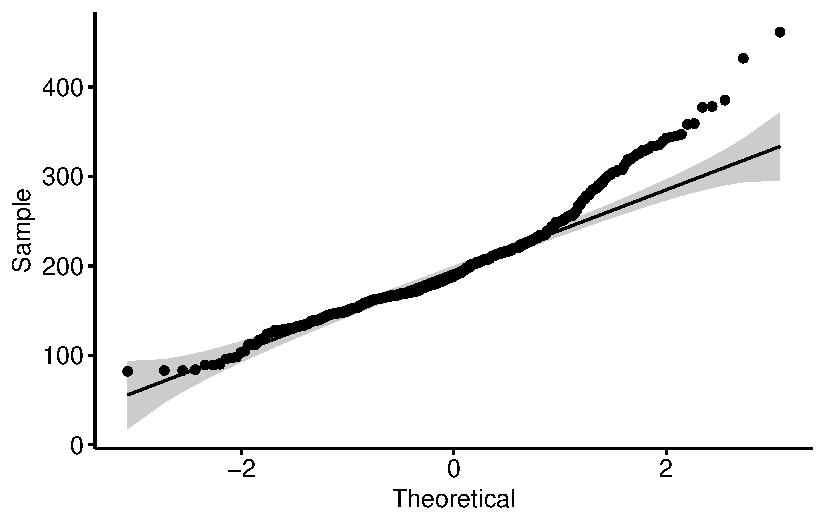
\includegraphics{_lin_reg1_files/figure-pdf/unnamed-chunk-30-1.pdf}

}

\end{figure}

\begin{Shaded}
\begin{Highlighting}[]
\NormalTok{df\_crit\_verb }\SpecialCharTok{|\textgreater{}} 
  \FunctionTok{filter}\NormalTok{(ff }\SpecialCharTok{\textgreater{}} \DecValTok{0}\NormalTok{) }\SpecialCharTok{|\textgreater{}} 
  \FunctionTok{mutate}\NormalTok{(}\AttributeTok{half =} \FunctionTok{if\_else}\NormalTok{(trial }\SpecialCharTok{\textgreater{}=} \DecValTok{104}\NormalTok{, }\StringTok{"1st"}\NormalTok{,}\StringTok{"2nd"}\NormalTok{)) }\SpecialCharTok{|\textgreater{}} 
\NormalTok{  ggpubr}\SpecialCharTok{::}\FunctionTok{ggqqplot}\NormalTok{( }\AttributeTok{x =} \StringTok{"ff"}\NormalTok{,}
                    \AttributeTok{color =} \StringTok{"half"}\NormalTok{)}
\end{Highlighting}
\end{Shaded}

\begin{figure}[H]

{\centering 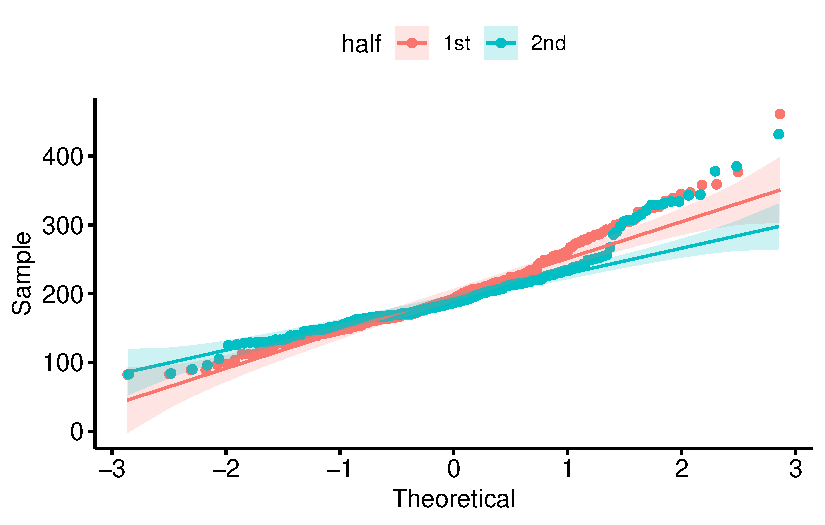
\includegraphics{_lin_reg1_files/figure-pdf/unnamed-chunk-31-1.pdf}

}

\end{figure}

\begin{Shaded}
\begin{Highlighting}[]
\NormalTok{df\_crit\_verb }\SpecialCharTok{|\textgreater{}} 
  \FunctionTok{filter}\NormalTok{(ff }\SpecialCharTok{\textgreater{}} \DecValTok{0}\NormalTok{) }\SpecialCharTok{|\textgreater{}} 
  \FunctionTok{mutate}\NormalTok{(}\AttributeTok{half =} \FunctionTok{if\_else}\NormalTok{(trial }\SpecialCharTok{\textgreater{}=} \DecValTok{104}\NormalTok{, }\StringTok{"1st"}\NormalTok{,}\StringTok{"2nd"}\NormalTok{)) }\SpecialCharTok{|\textgreater{}} 
\NormalTok{  ggpubr}\SpecialCharTok{::}\FunctionTok{ggqqplot}\NormalTok{( }\AttributeTok{x =} \StringTok{"ff"}\NormalTok{,}
                    \AttributeTok{color =} \StringTok{"half"}\NormalTok{,}
                    \AttributeTok{facet.by =} \StringTok{"px"}\NormalTok{)}
\end{Highlighting}
\end{Shaded}

\begin{figure}[H]

{\centering 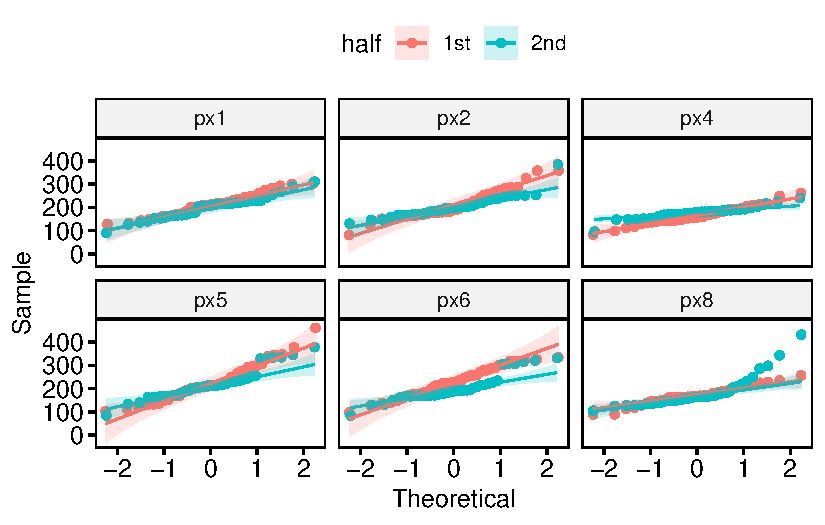
\includegraphics{_lin_reg1_files/figure-pdf/unnamed-chunk-32-1.pdf}

}

\end{figure}

\begin{Shaded}
\begin{Highlighting}[]
\FunctionTok{plot}\NormalTok{(}\FunctionTok{density}\NormalTok{(}\FunctionTok{resid}\NormalTok{(fit\_ff)))}
\end{Highlighting}
\end{Shaded}

\begin{figure}[H]

{\centering 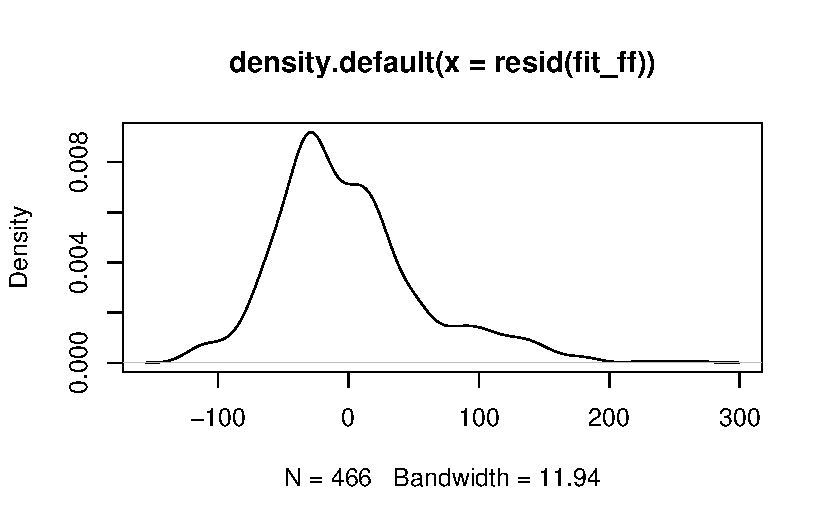
\includegraphics{_lin_reg1_files/figure-pdf/unnamed-chunk-33-1.pdf}

}

\end{figure}

\hypertarget{log-transformation}{%
\paragraph{Log transformation}\label{log-transformation}}

\begin{itemize}
\item
  for more see Section 5.4 in Winter (2019)
\item
  the R funtion \texttt{log()} computes the `natural logarithm' (and is
  the inverse of the exponential \texttt{exp()})
\item
  \texttt{log()} makes large numbers smaller
\item
  \texttt{exp()} makes small numbers larger
\end{itemize}

\begin{Shaded}
\begin{Highlighting}[]
\FunctionTok{log}\NormalTok{(}\DecValTok{0}\NormalTok{)}
\end{Highlighting}
\end{Shaded}

\begin{verbatim}
[1] -Inf
\end{verbatim}

\begin{Shaded}
\begin{Highlighting}[]
\FunctionTok{log}\NormalTok{(}\DecValTok{1}\SpecialCharTok{:}\DecValTok{10}\NormalTok{)}
\end{Highlighting}
\end{Shaded}

\begin{verbatim}
 [1] 0.0000000 0.6931472 1.0986123 1.3862944 1.6094379 1.7917595 1.9459101
 [8] 2.0794415 2.1972246 2.3025851
\end{verbatim}

\begin{Shaded}
\begin{Highlighting}[]
\FunctionTok{log}\NormalTok{(}\FunctionTok{c}\NormalTok{(}\DecValTok{10}\NormalTok{,}\DecValTok{20}\NormalTok{,}\DecValTok{30}\NormalTok{,}\DecValTok{40}\NormalTok{,}\DecValTok{100}\NormalTok{))}
\end{Highlighting}
\end{Shaded}

\begin{verbatim}
[1] 2.302585 2.995732 3.401197 3.688879 4.605170
\end{verbatim}

\begin{Shaded}
\begin{Highlighting}[]
\FunctionTok{exp}\NormalTok{(}\DecValTok{1}\SpecialCharTok{:}\DecValTok{10}\NormalTok{)}
\end{Highlighting}
\end{Shaded}

\begin{verbatim}
 [1]     2.718282     7.389056    20.085537    54.598150   148.413159
 [6]   403.428793  1096.633158  2980.957987  8103.083928 22026.465795
\end{verbatim}

\begin{Shaded}
\begin{Highlighting}[]
\FunctionTok{exp}\NormalTok{(}\FunctionTok{log}\NormalTok{(}\DecValTok{1}\SpecialCharTok{:}\DecValTok{10}\NormalTok{))}
\end{Highlighting}
\end{Shaded}

\begin{verbatim}
 [1]  1  2  3  4  5  6  7  8  9 10
\end{verbatim}

\hypertarget{log-transformation-1}{%
\paragraph*{Log transformation}\label{log-transformation-1}}
\addcontentsline{toc}{paragraph}{Log transformation}

\begin{itemize}
\tightlist
\item
  continuous variables truncated at 0 typically have a \emph{positive
  skew}

  \begin{itemize}
  \tightlist
  \item
    a lot of small values (e.g., \texttt{tt} \textless{} 500ms), with
    some larger values (\textgreater{} \texttt{tt} 1000)
  \item
    this usually means our residuals are also positively skewed, i.e.,
    not normally distributed
  \end{itemize}
\item
  so we typically log-transform raw reading/reaction times for our
  linear models
\end{itemize}

\begin{Shaded}
\begin{Highlighting}[]
\CommentTok{\# fit simple linear model with log}
\NormalTok{fit\_ff\_log }\OtherTok{\textless{}{-}}\NormalTok{ df\_crit\_verb }\SpecialCharTok{\%\textgreater{}\%}
  \FunctionTok{filter}\NormalTok{(ff }\SpecialCharTok{\textgreater{}} \DecValTok{0}\NormalTok{) }\SpecialCharTok{\%\textgreater{}\%} \CommentTok{\# important! you can\textquotesingle{}t log transform 0}
  \FunctionTok{lm}\NormalTok{(}\FunctionTok{log}\NormalTok{(ff) }\SpecialCharTok{\textasciitilde{}}\NormalTok{ lifetime, }\AttributeTok{data =}\NormalTok{ .)}
\FunctionTok{summary}\NormalTok{(fit\_ff\_log)}
\end{Highlighting}
\end{Shaded}

\begin{verbatim}

Call:
lm(formula = log(ff) ~ lifetime, data = .)

Residuals:
     Min       1Q   Median       3Q      Max 
-0.85247 -0.15738 -0.01522  0.15364  0.88707 

Coefficients:
            Estimate Std. Error t value            Pr(>|t|)    
(Intercept)  5.25882    0.01286 408.858 <0.0000000000000002 ***
lifetime1    0.02498    0.02572   0.971               0.332    
---
Signif. codes:  0 '***' 0.001 '**' 0.01 '*' 0.05 '.' 0.1 ' ' 1

Residual standard error: 0.2777 on 464 degrees of freedom
Multiple R-squared:  0.002029,  Adjusted R-squared:  -0.0001221 
F-statistic: 0.9432 on 1 and 464 DF,  p-value: 0.3319
\end{verbatim}

\hypertarget{communicating-your-results}{%
\section{Communicating your results}\label{communicating-your-results}}

\begin{itemize}
\tightlist
\item
  model summaries can be provided via tables and/or figures

  \begin{itemize}
  \tightlist
  \item
    you should always report the t-values and p-values of an effect
  \end{itemize}
\end{itemize}

\begin{Shaded}
\begin{Highlighting}[]
\NormalTok{df\_crit\_verb }\SpecialCharTok{|\textgreater{}} 
  \FunctionTok{filter}\NormalTok{(ff }\SpecialCharTok{\textgreater{}} \DecValTok{0}\NormalTok{) }\SpecialCharTok{|\textgreater{}} 
  \FunctionTok{mutate}\NormalTok{(}\AttributeTok{log\_ff =} \FunctionTok{log}\NormalTok{(ff)) }\SpecialCharTok{|\textgreater{}} 
  \FunctionTok{mutate}\NormalTok{(}\AttributeTok{half =} \FunctionTok{if\_else}\NormalTok{(trial }\SpecialCharTok{\textgreater{}=} \DecValTok{104}\NormalTok{, }\StringTok{"1st"}\NormalTok{,}\StringTok{"2nd"}\NormalTok{)) }\SpecialCharTok{|\textgreater{}} 
\NormalTok{  ggpubr}\SpecialCharTok{::}\FunctionTok{ggqqplot}\NormalTok{(}\AttributeTok{x =} \StringTok{"log\_ff"}\NormalTok{)}
\end{Highlighting}
\end{Shaded}

\begin{figure}[H]

{\centering 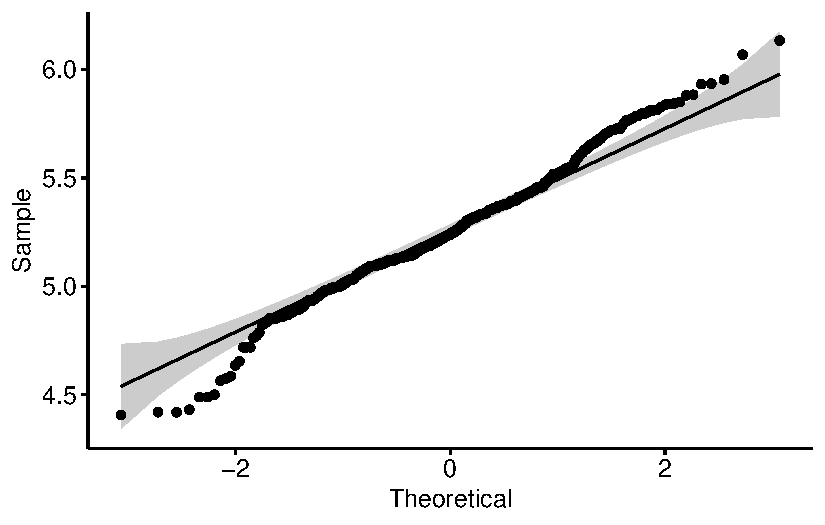
\includegraphics{_lin_reg1_files/figure-pdf/unnamed-chunk-37-1.pdf}

}

\end{figure}

\begin{Shaded}
\begin{Highlighting}[]
\NormalTok{df\_crit\_verb }\SpecialCharTok{|\textgreater{}} 
  \FunctionTok{filter}\NormalTok{(ff }\SpecialCharTok{\textgreater{}} \DecValTok{0}\NormalTok{) }\SpecialCharTok{|\textgreater{}} 
  \FunctionTok{mutate}\NormalTok{(}\AttributeTok{log\_ff =} \FunctionTok{log}\NormalTok{(ff)) }\SpecialCharTok{|\textgreater{}} 
  \FunctionTok{mutate}\NormalTok{(}\AttributeTok{half =} \FunctionTok{if\_else}\NormalTok{(trial }\SpecialCharTok{\textgreater{}=} \DecValTok{104}\NormalTok{, }\StringTok{"1st"}\NormalTok{,}\StringTok{"2nd"}\NormalTok{)) }\SpecialCharTok{|\textgreater{}} 
\NormalTok{  ggpubr}\SpecialCharTok{::}\FunctionTok{ggqqplot}\NormalTok{( }\AttributeTok{x =} \StringTok{"log\_ff"}\NormalTok{,}
                    \AttributeTok{color =} \StringTok{"half"}\NormalTok{)}
\end{Highlighting}
\end{Shaded}

\begin{figure}[H]

{\centering 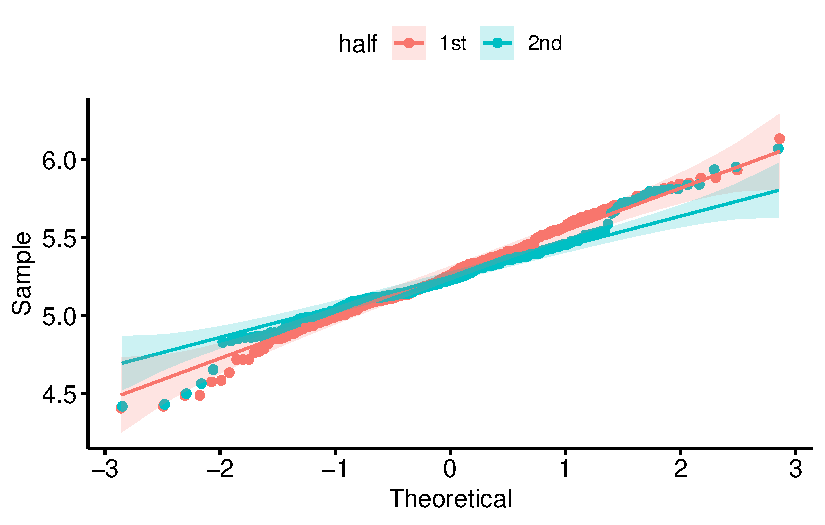
\includegraphics{_lin_reg1_files/figure-pdf/unnamed-chunk-38-1.pdf}

}

\end{figure}

\begin{Shaded}
\begin{Highlighting}[]
\NormalTok{df\_crit\_verb }\SpecialCharTok{|\textgreater{}} 
  \FunctionTok{filter}\NormalTok{(ff }\SpecialCharTok{\textgreater{}} \DecValTok{0}\NormalTok{) }\SpecialCharTok{|\textgreater{}} 
  \FunctionTok{mutate}\NormalTok{(}\AttributeTok{log\_ff =} \FunctionTok{log}\NormalTok{(ff)) }\SpecialCharTok{|\textgreater{}} 
  \FunctionTok{mutate}\NormalTok{(}\AttributeTok{half =} \FunctionTok{if\_else}\NormalTok{(trial }\SpecialCharTok{\textgreater{}=} \DecValTok{104}\NormalTok{, }\StringTok{"1st"}\NormalTok{,}\StringTok{"2nd"}\NormalTok{)) }\SpecialCharTok{|\textgreater{}} 
\NormalTok{  ggpubr}\SpecialCharTok{::}\FunctionTok{ggqqplot}\NormalTok{( }\AttributeTok{x =} \StringTok{"log\_ff"}\NormalTok{,}
                    \AttributeTok{color =} \StringTok{"half"}\NormalTok{,}
                    \AttributeTok{facet.by =} \StringTok{"px"}\NormalTok{)}
\end{Highlighting}
\end{Shaded}

\begin{figure}[H]

{\centering 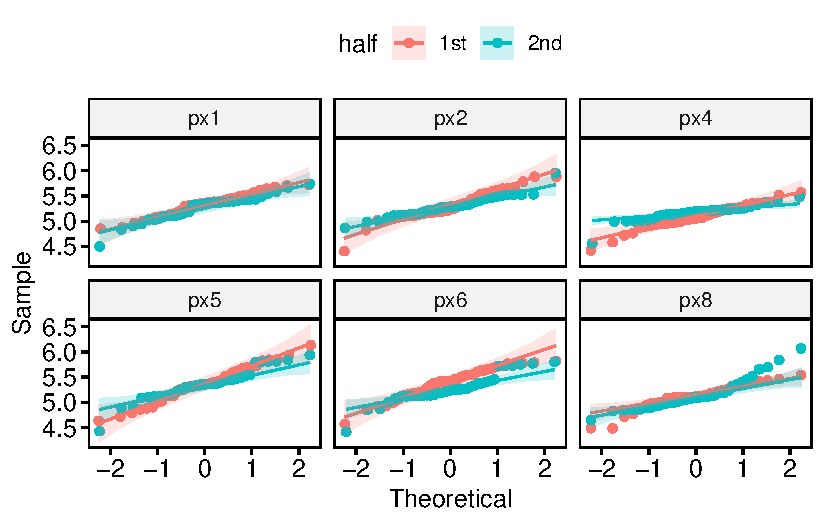
\includegraphics{_lin_reg1_files/figure-pdf/unnamed-chunk-39-1.pdf}

}

\end{figure}

\begin{Shaded}
\begin{Highlighting}[]
\FunctionTok{plot}\NormalTok{(}\FunctionTok{density}\NormalTok{(}\FunctionTok{resid}\NormalTok{(fit\_ff)))}
\end{Highlighting}
\end{Shaded}

\begin{figure}[H]

{\centering 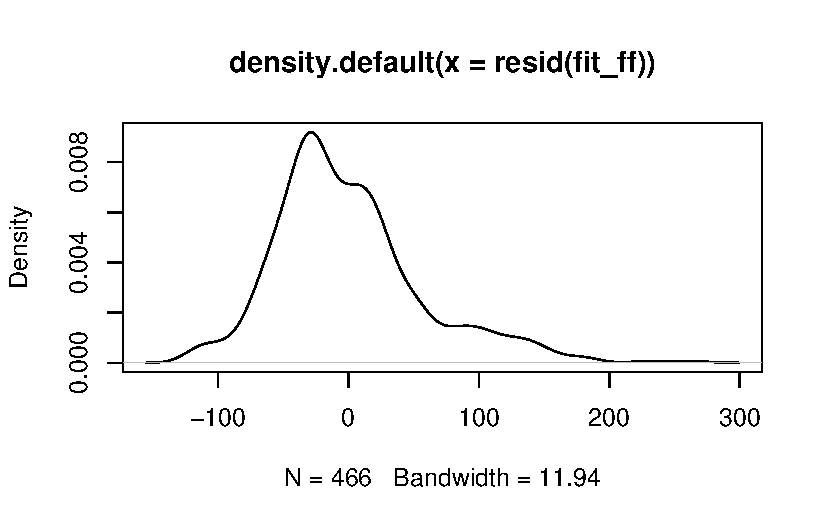
\includegraphics{_lin_reg1_files/figure-pdf/unnamed-chunk-40-1.pdf}

}

\end{figure}

\begin{Shaded}
\begin{Highlighting}[]
\NormalTok{b0 }\OtherTok{\textless{}{-}} \FunctionTok{coef}\NormalTok{(fit\_ff\_log)[}\StringTok{"(Intercept)"}\NormalTok{]}
\NormalTok{b1 }\OtherTok{\textless{}{-}}\NormalTok{ (}\FunctionTok{coef}\NormalTok{(fit\_ff\_log)[}\StringTok{"lifetime1"}\NormalTok{]) }

\FunctionTok{exp}\NormalTok{(b0}\SpecialCharTok{+}\NormalTok{b1)}
\end{Highlighting}
\end{Shaded}

\begin{verbatim}
(Intercept) 
   197.1179 
\end{verbatim}

\hypertarget{summary-1}{%
\section{Summary}\label{summary-1}}

\begin{itemize}
\item
  we saw that the equation for a straight line boils down to its
  intercept and slope
\item
  we fit our first linear model with a categorical predictor
\item
  next, we'll look at a case with more than one predictor:
  \textbf{multiple} regression
\end{itemize}

\hypertarget{important-terms}{%
\subsection*{Important terms}\label{important-terms}}
\addcontentsline{toc}{subsection}{Important terms}

\begin{longtable}[]{@{}
  >{\raggedright\arraybackslash}p{(\columnwidth - 2\tabcolsep) * \real{0.2917}}
  >{\raggedright\arraybackslash}p{(\columnwidth - 2\tabcolsep) * \real{0.7083}}@{}}
\toprule\noalign{}
\endhead
\bottomrule\noalign{}
\endlastfoot
dependent variable (DV) & outcome, measure, \(x\) \\
independent variable (IV) & predictor, fixed effect, \(y\) \\
equation for a straight line & \\
Simple regression & predicting outcome of a DV from an IV \\
Slope & change in \$y\$ (DV) associated with a unit change in \$x\$ (IV)
= 0 \\
Intercept & value of \$y\$ (DV) when \$x\$ (IV) = 0 \\
Normality assumption & \\
Residuals & \\
Coefficients & \\
Log-transformation & \\
\end{longtable}

\hypertarget{important-functions}{%
\subsection*{Important functions}\label{important-functions}}
\addcontentsline{toc}{subsection}{Important functions}

\begin{longtable}[]{@{}
  >{\raggedright\arraybackslash}p{(\columnwidth - 2\tabcolsep) * \real{0.5556}}
  >{\raggedright\arraybackslash}p{(\columnwidth - 2\tabcolsep) * \real{0.4444}}@{}}
\toprule\noalign{}
\endhead
\bottomrule\noalign{}
\endlastfoot
\texttt{lm(dv\ \textasciitilde{}\ 1\ +\ iv,\ data\ =\ df\_name)} &
simple linear model \\
\texttt{summary(model)} & print model summary \\
\texttt{coef(model)} & print coefficients (intercept, slope) \\
\texttt{log()} & log-transform a continuous variable \\
\end{longtable}

\hypertarget{session-info}{%
\section*{Session Info}\label{session-info}}

\begin{Shaded}
\begin{Highlighting}[]
\FunctionTok{sessionInfo}\NormalTok{()}
\end{Highlighting}
\end{Shaded}

\begin{verbatim}
R version 4.2.3 (2023-03-15)
Platform: aarch64-apple-darwin20 (64-bit)
Running under: macOS Ventura 13.2.1

Matrix products: default
BLAS:   /Library/Frameworks/R.framework/Versions/4.2-arm64/Resources/lib/libRblas.0.dylib
LAPACK: /Library/Frameworks/R.framework/Versions/4.2-arm64/Resources/lib/libRlapack.dylib

locale:
[1] en_US.UTF-8/en_US.UTF-8/en_US.UTF-8/C/en_US.UTF-8/en_US.UTF-8

attached base packages:
[1] stats     graphics  grDevices utils     datasets  methods   base     

other attached packages:
 [1] magick_2.7.4    broom_1.0.4     lubridate_1.9.2 forcats_1.0.0  
 [5] stringr_1.5.0   dplyr_1.1.1     purrr_1.0.1     readr_2.1.4    
 [9] tidyr_1.3.0     tibble_3.2.1    ggplot2_3.4.2   tidyverse_2.0.0

loaded via a namespace (and not attached):
 [1] httr_1.4.5        bit64_4.0.5       vroom_1.6.1       jsonlite_1.8.4   
 [5] viridisLite_0.4.1 splines_4.2.3     carData_3.0-5     here_1.0.1       
 [9] yaml_2.3.7        pillar_1.9.0      backports_1.4.1   lattice_0.20-45  
[13] glue_1.6.2        digest_0.6.31     ggsignif_0.6.4    rvest_1.0.3      
[17] colorspace_2.1-0  htmltools_0.5.5   Matrix_1.5-3      rbbt_0.0.0.9000  
[21] pkgconfig_2.0.3   scales_1.2.1      webshot_0.5.4     svglite_2.1.1    
[25] tzdb_0.3.0        timechange_0.2.0  mgcv_1.8-42       generics_0.1.3   
[29] farver_2.1.1      car_3.1-2         ggpubr_0.6.0      withr_2.5.0      
[33] cli_3.6.1         magrittr_2.0.3    crayon_1.5.2      evaluate_0.20    
[37] fs_1.6.1          fansi_1.0.4       nlme_3.1-162      rstatix_0.7.2    
[41] xml2_1.3.3        tools_4.2.3       hms_1.1.3         lifecycle_1.0.3  
[45] munsell_0.5.0     kableExtra_1.3.4  compiler_4.2.3    systemfonts_1.0.4
[49] rlang_1.1.0       grid_4.2.3        rstudioapi_0.14   labeling_0.4.2   
[53] rmarkdown_2.21    gtable_0.3.3      abind_1.4-5       curl_5.0.0       
[57] R6_2.5.1          knitr_1.42        fastmap_1.1.1     bit_4.0.5        
[61] utf8_1.2.3        rprojroot_2.0.3   stringi_1.7.12    parallel_4.2.3   
[65] Rcpp_1.0.10       vctrs_0.6.1       png_0.1-8         tidyselect_1.2.0 
[69] xfun_0.38        
\end{verbatim}

\hypertarget{references}{%
\section*{References}\label{references}}

\hypertarget{refs}{}
\begin{CSLReferences}{1}{0}
\leavevmode\vadjust pre{\hypertarget{ref-debruine_understanding_2021}{}}%
DeBruine, L. M., \& Barr, D. J. (2021). Understanding Mixed-Effects
Models Through Data Simulation. \emph{Advances in Methods and Practices
in Psychological Science}, \emph{4}(1), 251524592096511.
\url{https://doi.org/10.1177/2515245920965119}

\leavevmode\vadjust pre{\hypertarget{ref-field_discovering_2013}{}}%
Field, A., Miles, J., \& Field, Z. (2013). \emph{Discovering statistics
using R} (Vol. 50, Issue 04, pp. 2114-50-2114).
\url{https://doi.org/10.5860/choice.50-2114}

\leavevmode\vadjust pre{\hypertarget{ref-winter_linear_2013}{}}%
Winter, B. (2013). \emph{Linear models and linear mixed effects models
in R: Tutorial 1}.
\url{https://bodowinter.com/tutorial/bw_LME_tutorial1.pdf}

\leavevmode\vadjust pre{\hypertarget{ref-winter_very_2014}{}}%
Winter, B. (2014). \emph{A very basic tutorial for performing linear
mixed effects analyses (Tutorial 2)}.
\url{https://bodowinter.com/tutorial/bw_LME_tutorial2.pdf}

\leavevmode\vadjust pre{\hypertarget{ref-winter_statistics_2019}{}}%
Winter, B. (2019). \emph{Statistics for Linguists: An Introduction Using
R}. Routledge. \url{https://doi.org/10.4324/9781315165547}

\end{CSLReferences}



\end{document}
